\documentclass[14pt,a4paper]{article} 
\usepackage[margin=1in]{geometry} 
\usepackage[utf8]{inputenc} 
\usepackage[english, russian]{babel} 
\usepackage{amsmath} 
\usepackage{amsfonts}
\usepackage{tcolorbox} 
\usepackage{amssymb} 
\usepackage{amsthm} 
\usepackage{lastpage} 
\usepackage{fancyhdr} 
\usepackage{accents}
\usepackage{tabto}
\usepackage{multicol}
\usepackage{graphicx}
\usepackage{verbatim}
\usepackage{mathdots}
\usepackage{pstricks,pst-node}
\usepackage{alltt}

\parindent = 3em
\parskip = 0pt

\graphicspath{{picks/}}
\DeclareGraphicsExtensions{.png}


\begin{document}
    \begin{titlepage}
        \newpage
         \begin{center}
             {\bfseries \large ПРАВИТЕЛЬСТВО РОССИЙСКОЙ ФЕДЕРАЦИИ\\
             НАЦИОНАЛЬНЫЙ ИССЛЕДОВАТЕЛЬСКИЙ УНИВЕРСИТЕТ\\
             «ВЫСШАЯ ШКОЛА ЭКОНОМИКИ»}\\
             \vspace{1cm}
             {Факультет компьютерных наук\\
             Департамент программной инженерии}\\
             \vspace{6cm}
             {\bfseries \Large  ПРОГРАММА, ЗАМЕНЯЮЩАЯ ВСЕ ГЛАСНЫЕ БУКВЫ В ЗАДАННОЙ ASCII-СТРОКЕ
             ЗАГЛАВНЫМИ}\\
             \vspace{1cm}
             {\bfseries Пояснительная записка}
             \vspace{3cm}
         \end{center}

         \begin{flushright}
             Исполнитель\\
             Студент группы БПИ 196\\
             Судаков Дмитрий Юрьевич
         \end{flushright}
         \vfill
         \begin{center}
             {\bfseries Москва, 2020}
         \end{center}
    \end{titlepage}


    \newpage
    \tableofcontents


    \newpage
    \section{Постановка задачи}
    \par{
        Разработать программу, заменяющую все гласные буквы в заданной ASCII-строке заглавными. 
    }\\
    
    \newpage
    \section{Описание алгоритма}
    \par{
        Для решения поставленной задачи было заведено два массива со всеми строчными и прописными гласными английскими и русскими буквами в кодировке OEM-866 (Такая кодировка была выбрана, так как она установлена по умолчанию в консоли). Далее осуществлялся поиск каждого символа из исходной строки в массиве строчных букв, и если поиск был успешным, то он заменяется на элемент с таким же индексом из массива прописных букв.
    }
    \subsection{Описание методов}
    \subsubsection{strLen}
    \par{
        \begin{tabular}{rlp{10cm}}
            Аргументы : & string  & ссылка на строку, заканчивающуюся символом '\textbackslash0' длину которой надо посчитать.\\
            Возвращаемое значение : & \multicolumn{2}{p{10cm}}{В регистр eax помещается длина строки с учётом символа}
        \end{tabular}
    }

    \subsubsection{findInStr}{
        \begin{tabular}{rlp{10cm}}
            Аргументы : & string  & Ссылка на строку в которой будет поиск\\
            \hfill & len0  & Длина строки с учётом нуля в конце \\
            \hfill & char & Символ, который надо найти\\
            Возвращаемое значение : & \multicolumn{2}{p{11cm}}{В регистр eax помещается -1, если символ не найден, или его индекс в строке, если найден}
        \end{tabular}
    }

    \subsubsection{transformString}{
        \begin{tabular}{rlp{11cm}}
            Описание : & \multicolumn{2}{p{10cm}}{Метод заменят все гласные буквы в строке на их заглавные эквиваленты.}\\
            Аргументы : & string  & Ссылка на строку в которой надо заменить символы\\
            Возвращаемое значение : & \multicolumn{2}{p{11cm}}{Изменяется переданная строка}
        \end{tabular}
    }

    \subsection{Формат входных данных}\par{
        Вводится строка состоящая из символов в кодировке OEM-866 длиной до 256 символов. Все символы, которые будут напечатаны сверх заданного лимита будут проигнорированны.
    }

    \subsection{Формат выходных данных}\par{
        Выводится сообщение с считанной строкой до и после преобразования.
    }

    \newpage
    \section{Приложение 1. Код программы}
    \begin{verbatim}
;Develop a program that replaces all
;vowels in a given ASCII string
;in capital

format          PE console 4.0
entry           start

include         'win32a.inc' 
 
section         '.code' code readable executable
 
  start:
    cinvoke printf, outEnterMessage         ;print message for user
    cinvoke scanf, inStringTemp, myStr      ;read users string	
    cinvoke printf, endl                    ;go to next line

    cinvoke printf, outStringBefore, myStr  ;print users line

    stdcall transformString, myStr          ;tranform string
	
    cinvoke printf, outStringAfter, myStr   ;print transformed string



  exit:
    cinvoke _getch

    invoke  ExitProcess, 0

;///////////////////////////////////////////////////////////////////////

;Function compute length of string, uncluding zero-symbol in the end
;Returns result in eax
proc strLen uses ecx edi, string
    xor al, al          ;clear al for comparing with string elems
    mov ecx, -1         ;ecx = -1 because if rep-cycle decrement ecx and stopped when ecx = 0

    mov edi, [string]   ;set edi on first element of our string
    cld                 ;set DF for scasb command

    repnz scasb         ;while ([edi] != al) {edi++; ecx--}

                        ;now ecx = -1 -(len+1) = -len-2
    not ecx             ;ecx = len+1
    mov eax, ecx        ;return result with eax

    ret
endp

;///////////////////////////////////////////////////////////////////////

;Fuction try to find number of given char in string
;Returns in eax number of char, or -1 if it hasn't found
proc findInStr uses ebx ecx edi, string, len0, char

    mov ecx, [len0]         ;ecx = len + 1
    mov ebx, [len0]         ;ebx = len + 1
    dec ebx				    ;ebx = len

    mov al, BYTE[char]      ;set to al our char
    mov edi, [string]       ;set edi on first element of our string
    cld                     ;set DF for scasb command

    repnz scasb             ;while ([edi] != al) {edi++; ecx--}

                            ;now in ecx number of char from the end
    test ecx, ecx           ;compare ecx with 0			
    mov eax, -1             ;if it equal to 0, set eax to -1  
    jz @f                   ;jump to the end of proc

    mov eax, ebx            ;eax = len
    sub eax, ecx            ;eax = number of our char
@@:
    ret
endp

;///////////////////////////////////////////////////////////////////////

;Method transformed all lowwercase vowels to uppercase
proc transformString uses eax ecx esi, string

    stdcall strLen, [string         ;eax = len + 1
    mov ecx, eax                    ;ecx = len + 1
    dec ecx                         ;ecx = len

    test ecx, ecx                   ;if string empty jump to the end
    je .exit	

    mov esi, [string]               ;set to esi adress of given string
    cld                             ;set DF for lodsb command
	
.forLoop:	
    xor eax, eax                    ;clear eax	
    lodsb                           ;move next symbol to al 
    stdcall findInStr, fromString, [fromStringLen0], eax
                                    ;find this symbol in fromString
    cmp eax, -1                     ;if eax == -1 go to the next symbol
    je @f

    dec esi                         ;back to prev symbol
    mov al, BYTE[toString+eax]      ;move to al capital leter
    mov [esi], al                   ;move to [esi] our letter
    inc esi                         ;move esi to the next symbol

@@:
    loop .forLoop
    
.exit:
    ret
endp

;///////////////////////////////////////////////////////////////////////

section         '.data' data readable writeable
    outEnterMessage         db 	'Enter Your string (no more than 255 symbols): ', 0
    inStringTemp            db	'%255[^',0Ah,']', 0
    endl                    db	10,13,0
    outStringBefore         db	'String before : %s', 10, 13, 0
    outStringAfter          db	'String after : %s', 10, 13, 0

    myStr                   db	256 dup(0)

    fromString              db 	'аеёиоуыэюяaeiouy',0            ;lowwercase letters
    fromStringLen0          dd	17	
    toString                db 	'АЕЁИОУЫЭЮЯAEIOUY',0            ;uppercase letters

section         '.idata' import data readable writeable
 
library         kernel32,'KERNEL32.DLL',\
                msvcrt, 'msvcrt.dll'
 
import          kernel32,\ 
                ExitProcess,'ExitProcess'

import          msvcrt,\
                __getmainargs,'__getmainargs',\
                fopen,'fopen',\
                fseek,'fseek',\
                ftell,'ftell',\
                malloc,'malloc',\
                free,'free',\
                fread,'fread',\
                fclose,'fclose',\
                printf,'printf',\
                scanf,'scanf',\
                _getch,'_getch',\
                puts,'puts'
    \end{verbatim}
     
    \section{Приложение 2. Тестирование программы}\par{
        \parindent = 0pt
        \parskip = 0.5cm
        Сначала попробуем ввести пустую строку :\\
        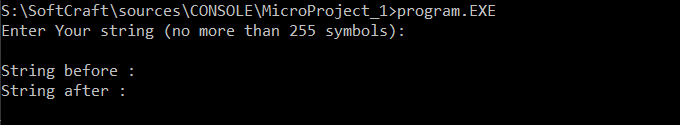
\includegraphics[width=175mm]{Test_0}\\
        
        Теперь попробуем превысить лимит символов :\\
        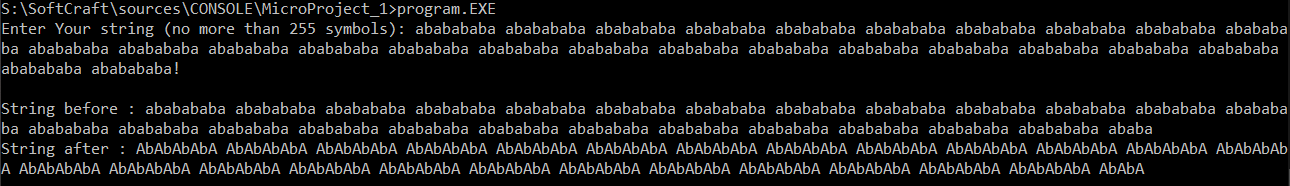
\includegraphics[width=175mm]{Test_1}\\
        Как можно видеть, последние символы обрезалить.\\

        Попробуем русский текст :\\
        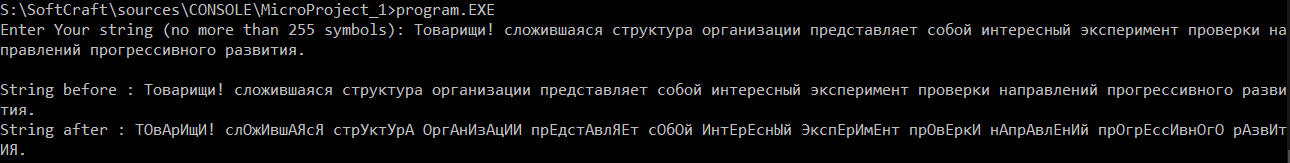
\includegraphics[width=175mm]{Test_2}\\

        Попробуем английский текст : \\
        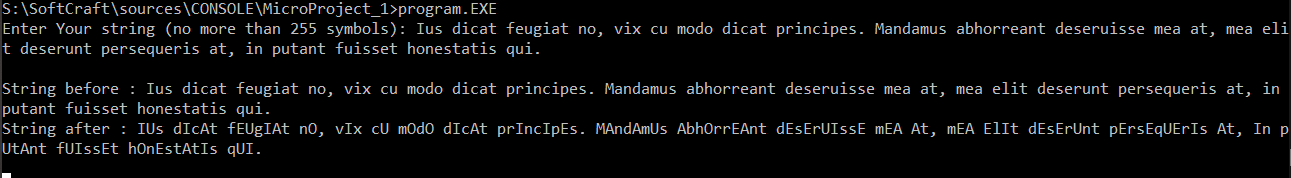
\includegraphics[width=175mm]{Test_3}\\

        Попробуем комбинированный текст :\\
        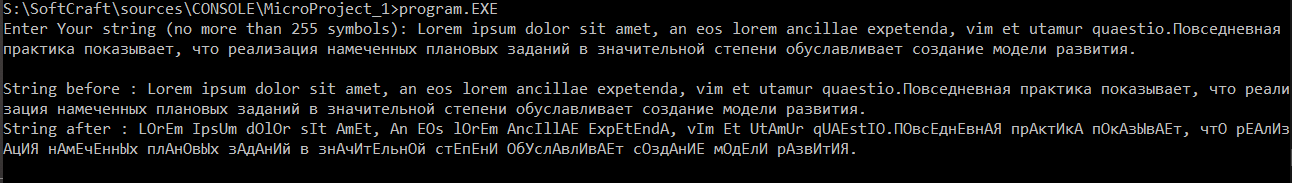
\includegraphics[width=175mm]{Test_4}

        Попробуем цифры и другие символы :\\
        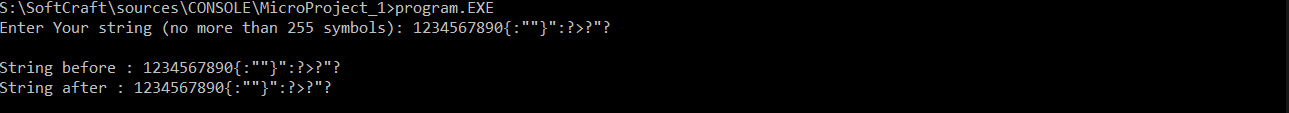
\includegraphics[width=175mm]{Test_5.png}
    }
    
\end{document}